\documentclass{article}

    \usepackage{fancyhdr}
    \usepackage{extramarks}
    \usepackage{amsmath}
    \usepackage{amsthm}
    \usepackage{amsfonts}
    \usepackage{tikz}
    \usepackage{amssymb}
    \usepackage{subcaption}
    \usetikzlibrary{decorations.markings}
    \tikzstyle{vertex}=[circle, draw, inner sep=0pt, minimum size=6pt]
    \newcommand{\vertex}{\node[vertex]}

    
    \usepackage{amsmath}
    \usepackage{algorithm}
    \usepackage[noend]{algpseudocode}
    
    \usepackage[utf8]{inputenc}
    \usepackage{enumerate}
    \usepackage{geometry}
    \usepackage{mathtools}
    \usepackage{parskip}
    \usepackage{xifthen, xparse}
    
    \algdef{SE}[SUBALG]{Indent}{EndIndent}{}{\algorithmicend\ }%
    \algtext*{Indent}
    \algtext*{EndIndent}
    
    
    
    \usetikzlibrary{automata,positioning}
    
    %
    % Basic Document Settings
    %
    
    \topmargin=-0.45in
    \evensidemargin=0in
    \oddsidemargin=0in
    \textwidth=6.5in
    \textheight=9.0in
    \headsep=0.25in
    
    \linespread{1.1}
    
    \pagestyle{fancy}
    \lhead{\hmwkAuthorName}
    \chead{\hmwkClass\ \hmwkTitle}
    \rhead{\firstxmark}
    \lfoot{\lastxmark}
    \cfoot{\thepage}
    
    \renewcommand\headrulewidth{0.4pt}
    \renewcommand\footrulewidth{0.4pt}
    
    \setlength\parindent{0pt}
    
    %
    % Create Problem Sections
    %
    
    \newcommand{\enterProblemHeader}[1]{
        \nobreak\extramarks{}{Problem \arabic{#1} continued on next page\ldots}\nobreak{}
        \nobreak\extramarks{Problem \arabic{#1} (continued)}{Problem \arabic{#1} continued on next page\ldots}\nobreak{}
    }
    
    \newcommand{\exitProblemHeader}[1]{
        \nobreak\extramarks{Problem \arabic{#1} (continued)}{Problem \arabic{#1} continued on next page\ldots}\nobreak{}
        \stepcounter{#1}
        \nobreak\extramarks{Problem \arabic{#1}}{}\nobreak{}
    }
    
    \newcommand\rowop[1]{\scriptstyle\smash{\xrightarrow[\vphantom{#1}]{\mkern-4mu#1\mkern-4mu}}}
    
    \DeclareDocumentCommand\converttorows%
    {>{\SplitList{,}}m}%
    {\ProcessList{#1}{\converttorow}}
    \NewDocumentCommand{\converttorow}{m}
    {\ifthenelse{\isempty{#1}}{}{\rowop{#1}}\\}
    
    \DeclareDocumentCommand \rowops{m}
    {\;
     \begin{matrix}
    \converttorows {#1}
     \end{matrix}
     \; }
    
    \setcounter{secnumdepth}{0}
    \newcounter{partCounter}
    \newcounter{homeworkProblemCounter}
    \setcounter{homeworkProblemCounter}{1}
    \nobreak\extramarks{Problem \arabic{homeworkProblemCounter}}{}\nobreak{}
    
    %
    % Homework Problem Environment
    %
    % This environment takes an optional argument. When given, it will adjust the
    % problem counter. This is useful for when the problems given for your
    % assignment aren't sequential. See the last 3 problems of this template for an
    % example.
    %
    \newenvironment{homeworkProblem}[1][-1]{
        \ifnum#1>0
            \setcounter{homeworkProblemCounter}{#1}
        \fi
        \section{Problem \arabic{homeworkProblemCounter}}
        \setcounter{partCounter}{1}
        \enterProblemHeader{homeworkProblemCounter}
    }{
        \exitProblemHeader{homeworkProblemCounter}
    }
    
    %
    % Homework Details
    %   - Title
    %   - Due date
    %   - Class
    %   - Section/Time
    %   - Instructor
    %   - Author
    %
    
    \newcommand{\hmwkTitle}{SOFTENG250 Assignment \#2}
    \newcommand{\hmwkClass}{D.S. and Algorithms}
    \newcommand{\hmwkAuthorName}{\textbf{Nisarag Bhatt}}

    
    %
    % Title Page
    %
    
    \title{
        \vspace{2in}
        \textmd{\textbf{\hmwkClass:\ \hmwkTitle}}\\
        \vspace{3in}
    }
    
    \author{\hmwkAuthorName}
    \date{}
    
    \renewcommand{\part}[1]{\textbf{\large Part \Alph{partCounter}}\stepcounter{partCounter}\\}
    
    %
    % Various Helper Commands
    %
    
    % Useful for algorithms
    \newcommand{\alg}[1]{\textsc{\bfseries \footnotesize #1}}
    
    % For derivatives
    \newcommand{\deriv}[1]{\frac{\mathrm{d}}{\mathrm{d}x} (#1)}
    
    % For partial derivatives
    \newcommand{\pderiv}[2]{\frac{\partial}{\partial #1} (#2)}
    
    % Integral dx
    \newcommand{\dx}{\mathrm{d}x}
    
    % Alias for the Solution section header
    \newcommand{\solution}{\textbf{\large Solution}}
    
    % Probability commands: Expectation, Variance, Covariance, Bias
    \newcommand{\E}{\mathrm{E}}
    \newcommand{\Var}{\mathrm{Var}}
    \newcommand{\Cov}{\mathrm{Cov}}
    \newcommand{\Bias}{\mathrm{Bias}}
    
    \begin{document}
    
    
    
    \pagebreak

    \begin{center}
        \textbf{Running Time}
    \end{center}
    
    \begin{homeworkProblem}
    
    Consider Euclidean algorithm. The input integers $n$ and $m$ are given in their decimal representations.
     
    \textbf{Part A}
     
    What is the size of the input for the algorithm?
    
    \textbf{Solution:}

    The initial size of the input of the algorithm would be the sum of the number of digits of $m$ and $n$.

    Or mathematically we could say Input $= (\lfloor{\log(m)}\rfloor + 1) + (\lfloor{\log(n)}\rfloor + 1)$
    
    
    \textbf{Part B}

    Explain why the running time of the algorithm is linear on the size of the input. For the analysis, assume that the division process takes a constant amount of time.

    \textbf{Solution:}

    Let's assume the worst case scenario: Where $n \neq m$ and $n > m$

    After two iterations of the algorithm, the input changes as such: $$\text{gcd}(n,m) \to \text{gcd}(m, n ~\text{mod}~ m) \to \text{gcd}(n ~\text{mod}~ m, m ~\text{mod}~ (n ~\text{mod}~ m) ) $$

    Also note that our first parameter changes from $n \to n~\text{mod}~m$ after $2$ iterations.

    Let's look at a single iteration of our algorithm:  
    
    Case 1: If $\left(m < \frac{n}{2}\right)$ , then $n~\text{mod}~m < m$ which is less than $\frac{n}{2}$.

    Case 2: If $\left(m > \frac{n}{2}\right)$ , then $n~\text{mod}~m = n - m$ which is less than $\frac{n}{2}$.

    In general, this means after any two consecutive iterations, both of the input arguments $n$ and $m$ must at least be halved in value. 
    
    This shows a logarithmic decrease in input size $(\lfloor{\log(m)}\rfloor + 1) + (\lfloor{\log(n)}\rfloor + 1)$ and the algorithm runs relative to the input size. Therefore this proves a linear upper bound of $\mathcal{O}(n) $, where $n$ here represent the total input size.
    
    \end{homeworkProblem}

    \pagebreak
    
    \begin{homeworkProblem}
    Let $p$ be a polynomial with positive coefficients. Show that $p$ is $\mathcal{O}(n^{\log(n)})$.
    
    \textbf{Solution:}

    Suppose $p=a_0 + a_1 n + a_2 n^2 + ... + a_i n^i$ then consider $\frac{p}{n^{\log(n)}}$ if we can 
    show that $\lim_{n \to \infty} \frac{p}{n^{\log(n)}} = 0$ then we are done so let's try to prove that.
    \begin{align*}
        L &= \lim_{n \to \infty}\frac{p}{n^{\log n}} \\
        L &= \lim_{n \to \infty} \frac{a_0 + a_1 n + a_2 n^2 + ... + a_i n^i}{n^{\log n}} \\
        L &= \lim_{n \to \infty} \frac{a_0}{n^{\log n}} + \frac{a_1}{n^{\log n - 1}} + \frac{a_2}{n^{\log n - 2}} + ... + \frac{a_i}{n^{\log n - i}} \\
    \end{align*}
    Now since all fractions have constants in the numerator and $n^{\text{log(n) - i}}$ in the denominator if we take the
    limit as ${n \to \infty}$ (for a sufficient $\log(n)>i$ or $n > 10^{i}$), we will always have the case that the denominator is larger than the numerator and this will
    grow much faster, so each fraction will tend to $0$ and therefore $L=0$. And by the definition of Big-Oh we have that: $p=\mathcal{O}(n^{\log(n)})$.
    \end{homeworkProblem}

    \begin{homeworkProblem}
    
    Show that $\sum^{n}_{i=1} i^2 = \Theta(n^3)$

    \textbf{Solution:}

    If we can prove that $\lim_{n \to \infty}\frac{\sum\limits^{n}_{i=1} i^2}{n^3} = C$ where $C>0$ then we are done since that is the
    definition of Big-Theta.

    Since it is a known fact that $\sum\limits^{n}_{i=1} i^2 = \frac{n(n+1)(2n+1)}{6} = \frac{n^3}{3} + \frac{n^2}{2} + \frac{n}{6}$ so now we try prove the limit:
    \begin{align*}
        L &= \lim_{n \to \infty}\frac{\sum\limits^{n}_{i=1} i^2}{n^3} \\
        L &= \lim_{n \to \infty}\frac{ \frac{n^3}{3} + \frac{n^2}{2} + \frac{n}{6}}{n^3}\\
        L &= \lim_{n \to \infty}\frac{1}{3} + \frac{1}{2n} + \frac{1}{6n^2} \\
        L &= \frac{1}{3} \\
    \end{align*}
    Since $L=\frac{1}{3}$ which is a non-negative constant we are done. Therefore $\sum\limits^{n}_{i=1} i^2 = \Theta(n^3)$.
    \end{homeworkProblem}

    \pagebreak

    \begin{homeworkProblem}
        Show that $n \log(n) = \Omega(\log(n!))$.

        \textbf{Solution:}

        To prove $n \log(n) = \Omega(\log(n!))$ we can show that $n \log(n) \geq c \log(n!)$ or we can equivalently prove 
        $n \log(n) \geq \log(n!)$.

        However since $\log(x)$ is an increasing function we can equivalently show that $\log(n^n) \geq \log(n!)$ or $n^n \geq n!$.

        Therefore we can prove this by induction (for $n>0$): 

        \textbf{Base Case}: $n^n \geq n! \Leftrightarrow 1^1 \geq 1! \Leftrightarrow 1 \geq 1 ~~ \checkmark$ 

        \textbf{Induction Case}: Assume $P(k)$ is true: $k^k \geq k!$

        Show $P(k+1)$ is true: $(k+1)^{k+1} \geq (k+1)!$
        \begin{align*}
            (k+1)! &= (k+1) \cdot (k) \cdot (k-1)...(3) \cdot (2) \cdot (1) \\
                   &= (k+1) \cdot (k!) \\
                   &\leq (k+1) \cdot k^k ~~~~ \text{By hypothesis}\\
                   &\leq (k+1) \cdot (k+1)^k ~~~~ \text{Since}~k+1 > k \\
                   &= (k+1)^{k+1} \\
        \end{align*}
        Therefore we can conclude by induction that: $n \log(n) \geq c \log(n!)$ is true for $n>0$ and by definition of Big Omega we are done.
    \end{homeworkProblem}

    \begin{homeworkProblem}
    Show that $a^n = \mathcal{O}(n!)$ for any positive integer $a > 1$.

    \textbf{Solution}

    To prove that $a^n = \mathcal{O}(n!)$ we must have that $a^n \leq c \cdot n!$ so if we can prove that 
    $n!$ grows faster than $a^n$ then we are done. 

    We can first consider the series $S = \sum\limits_{n=0}^{\infty} \frac{a^n}{n!}$ if this series converges to $0$ we are done. 

    Now consider the ratio test for series: Consider $t_n=\frac{a^n}{n!}$ then 
    \begin{align*}
        \frac{t_{n+1}}{t_n} &=\frac{a^{n+1}}{(n+1)!} \cdot \frac{n!}{a^n} = \frac{a}{n+1} \\
        \therefore \lim_{n \to \infty}  \frac{a}{n+1} &= 0
    \end{align*}

    Hence we can conclude $n!$ grows much faster than $a^n$ and because of this we can conclude that after a certain value the function $n!$ will surpass $a^n$ and therefore $a^n = \mathcal{O}(n!)$.

    \end{homeworkProblem}

    \pagebreak

    \begin{homeworkProblem}
    Show that $\sum\limits_{i=1}^n \log\left(\frac{n}{i}\right) = \Theta(n)$

    If we can prove that $\lim_{n\to \infty} \frac{\sum\limits_{i=1}^n \log\left(\frac{n}{i}\right)}{n} = c$ where $c>0$ then we are done since that is the definition of big-theta.
    So let's attempt to do that.

    \begin{align*}
        \sum\limits_{i=1}^n \log\left(\frac{n}{i}\right) &= \sum\limits_{i=1}^n \log(n) - \log(i) \\
        \sum\limits_{i=1}^n \log\left(\frac{n}{i}\right) &= (\log(n)-\log(1)) + (\log(n) - \log(2)) + (\log(n) - \log(3)) + ... +(\log(n) - \log(n)) \\
        \sum\limits_{i=1}^n \log\left(\frac{n}{i}\right) &= \underbrace{\log(n) + \log(n) + \log(n) + ... + \log(n)}_{n} - (\log(1) + \log(2) + \log(3) + ... + \log(n)) \\
        \sum\limits_{i=1}^n \log\left(\frac{n}{i}\right) &= n \log(n) - \log(n!) \\
        \sum\limits_{i=1}^n \log\left(\frac{n}{i}\right) &= \log\left(\frac{n^n}{n!}\right) \\
    \end{align*}
    Now consider:
    \begin{align*}
        L &= \lim_{n \to \infty} \frac{\sum\limits_{i=1}^n \log\left(\frac{n}{i}\right)}{n}\\
        L &= \lim_{n \to \infty} \frac{\log\left(\frac{n^n}{n!}\right)}{n} \\
        L &= \lim_{n \to \infty} \frac{\log\left(\frac{(n+1)^{n+1}}{(n+1)!}\right) - \log\left(\frac{n^n}{n!}\right)}{(n+1)-(n)}  ~~~~ \text{Using Stolz-Cesaro}\\ 
        L &= \lim_{n \to \infty}\log\left(\frac{(n+1)^{n+1}}{(n+1)!}\frac{n!}{n^n}\right) \\
        L &= \lim_{n \to \infty} \log\left( \frac{(n+1)^{n+1}}{n^n}  \cdot \frac{1}{n+1} \right) \\
        L &= \lim_{n \to \infty} \log \left(1+\frac1n\right)^n \\
        L &= \log(e) ~~~ \text{Assuming log is natural log}\\
        L &= 1 \\
    \end{align*}    

    Since we have proved that $\lim_{n\to \infty} \frac{\sum\limits_{i=1}^n \log\left(\frac{n}{i}\right)}{n} = 1$ we are done due to the definition of Big-Theta.

    $\therefore$ $\sum\limits_{i=1}^n \log\left(\frac{n}{i}\right) = \Theta(n)$ \qed
    \end{homeworkProblem}

    \pagebreak
    \begin{homeworkProblem}

    For the codes below analyse the running times in terms of $\Theta$ notation.

        \begin{algorithm}
            \caption{}\label{euclid}
            \begin{algorithmic}[1]
                \State For $i=1$ to $n$ do
                    \Indent 
                        \State $j = n - i$
                        \State while $j \geq 0$ do 
                        \Indent
                            \State $j=j-3$
                        \EndIndent
                    \EndIndent
            \end{algorithmic}
        \end{algorithm}
        Analysis: Outer Loop $(i)$ in each iteration: $1,2,3,...,n-1$

                  Inner Loop $(j)$ in each iteration: $\frac{n-1}{3},\frac{n-2}{3},\frac{n-3}{3},...,1 = \left(\frac{n}{3} - \frac{1}{3} \right), \left(\frac{n}{3} - \frac{2}{3} \right), \left(\frac{n}{3} - \frac{3}{3} \right),...,1$

                  Updating $j$ takes constant time.

                  Sum: $T(n)=(n)\left(\frac{n}{3} - k \right) = \frac{n^2}{3} - kn = \boxed{\Theta(n^2)}$
        \begin{algorithm}
            \caption{}\label{euclid}
            \begin{algorithmic}[1]
                \State Set $s=0$
                    \Indent 
                        \State For $i=1$ to $n$ do
                        \Indent
                            \State For $j=3 \cdot i$ to $n$ do
                            \Indent
                                \State $s=s+1$
                            \EndIndent
                        \EndIndent
                    \EndIndent
            \end{algorithmic}
        \end{algorithm}

        For this algorithm we can determine the run time mathematically:
        \begin{align*}
            T(n) &=  \sum\limits_{i=1}^{n} \sum\limits_{j=3i}^{n} c = c \sum\limits_{i=1}^{n} \sum\limits_{j=3i}^{n} 1 =c \sum\limits_{i=1}^{n} (n-3i+1) = c(n+1) \sum\limits_{i=1}^{n} 1 - 3 \sum\limits_{i=1}^{n} i \\
            T(n) &= c(n+1)(n) - 3 \left(\frac{n(n+1)}{2} \right) = (n^2+n) \cdot \left(c - \frac{3}{2}\right) = k(n^2+n) = \boxed{\Theta (n^2)}\\ 
        \end{align*}
        This is because we have $2$ for loops and each $i$,$j$ are incrementing by $1$ and updating $s$ takes a constant time hence the $c$ inside the series.
        \begin{algorithm}
            \caption{}\label{euclid}
            \begin{algorithmic}[1]
                \State For $i=1$ to $n$ do
                    \Indent 
                        \State $j = i$
                        \State while $j < n$ do 
                        \Indent
                            \State $j=2 \cdot j$
                        \EndIndent
                    \EndIndent
            \end{algorithmic}
        \end{algorithm}

        Analysis: Outer Loop $(i)$ in each iteration: $1,2,3,...,n$

        Updating $j$ takes constant time.

        Inner Loop $(j)$ in each iteration: $\log(n)$, $\log(n)-\log(2)$, $\log(n)-\log(3)$,..,$0$ which is equivalent to $\log(n)$, $\log\left(\frac{n}{2}\right)$, $\log\left(\frac{n}{3}\right), ...,0$. So $\log(n)-\log(i)$ = start the loop from number $i$ as when $i$ gets larger, the number of multiplication before $j$ reaches $n$ will decrease logarithmically.
        
        And since $\sum\limits_{i=1}^n \log\left(\frac{n}{i}\right) = \Theta(n)$ (from problem 6) we have that $T(n) = \boxed{\Theta(n)}.$
    \end{homeworkProblem}

    \pagebreak
    
    \begin{center}
        \textbf{Graphs}
    \end{center}

    \begin{homeworkProblem}
        Let $G$ be any graph. Explain why the sum of all degrees of the vertices of any graph $G$ equals twice the number of edges of $G$.

        \textbf{Solution:}

        Let $e\in E(G)$ by any edge, then we can say $e$ connects $2$ vertices together. By adding another edge to the graph $G$, $1$ degree
        must be added to each vertex the edge connects to (i.e. if vertex $A$ is connected to vertex $B$ then vertex $B$ must be connected to vertex $A$) and
        thus the sum increases by $2$. Therefore $\sum\limits_{V \in V(G)} deg(V) = 2 |E(G)|$.
    \end{homeworkProblem}

    \begin{homeworkProblem}
        How many edges does a complete bipartite graph $K_{n,m}$ have?

        \textbf{Solution:}
        A complete bipartite graph has $m \cdot n$ edges.
    \end{homeworkProblem}

    \begin{homeworkProblem}
        Prove that if there is a path in a graph from vertex $x$
        to vertex $y$ and $x \neq y$ then there is a simple path from $x$ to $y$. 
        Recall that simple path is a path in which every vertex appears at most once.

        \textbf{Solution:}
        If a vertex appears more than once on the path from $x$ to $y$, that means that there is a cycle in that path and if there is a cycle we can remove all the nodes in that cycle.

        For example consider the path: $\{x \to c_1 \to c_2 \to c_3 \to c_4 \to c_1 \to y \}$, there is a cycle in this path: $C = \{c_1 \to c_2 \to c_3 \to c_4 \to c_1 \}$ since we can simply remove this cycle from our path we can 
        thus reduce our path to a simple path which is just $\{x \to c_1 \to y \}$

        If we have more cycles we can repeat this process. Since there can only be a finite amount of nodes at a certain time after we have completed removing all the cycles, we will have a path between $x$ and $y$ that which does not contain a cycle
        and hence a simple path.

    \end{homeworkProblem}

    \begin{homeworkProblem}
        Show that every finite connected graph $G$ with more than $1$ vertex has two vertices of the same degree.

        \textbf{Solution:}

        As the graph is connected, no vertex can have a degree of $0$ and at most a vertex can have is a degree of $n-1$ which means it is connected to every other vertex. 

        Let's use a proof by contradiction to prove this:

        If vertex 1 has a degree of 1 and vertex 2 has a degree of 2... 
        At vertex $n-1$, it will have a degree of $(n-1)$. However, at the last vertex $n$, it cannot have a degree of $n$ as vertices cannot connect to itself in an undirected graph which means vertex $n$ has at most $n-1$ degrees. 
        This proves that it will have the same degree as one of the previous vertices. 

        A contradiction to our initial assumption is found, therefore in graph $G$, at least two vertices must have the same degree. 
    \end{homeworkProblem}

    \begin{homeworkProblem}
        We call a graph $3$-regular if every vertex of the graph has degree $3$. Draw $3$-regular connected graphs consisting of $4$ vertices, $6$ vertices, and $8$ vertices.

        \textbf{Solution:}

        I have drawn them below respectively:
        \begin{center}
        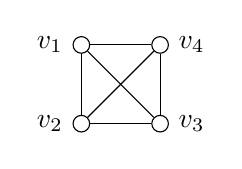
\begin{tikzpicture}
            \vertex (v2) at (0,0) [label=left:$v_2$]{};
            \vertex (v1) at (0,1) [label=left:$v_1$]{};
            \vertex (v4) at (1,1) [label=right:$v_4$]{};
            \vertex (v3) at (1,0) [label=right:$v_3$]{};
            \path 
                (v1) edge (v2)
                (v2) edge (v3)
                (v3) edge (v4)
                (v4) edge (v1)
                (v1) edge (v3)
                (v2) edge (v4)
            ;
        \end{tikzpicture}
        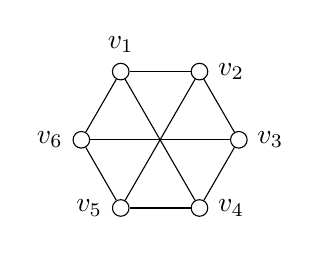
\begin{tikzpicture}
            \vertex (v1) at (120:1) [label=above:$v_1$]{};
            \vertex (v2) at (60:1) [label=right:$v_2$]{};
            \vertex (v3) at (360:1) [label=right:$v_3$]{};
            \vertex (v4) at (300:1) [label=right:$v_4$]{};
            \vertex (v5) at (240:1) [label=left:$v_5$]{};
            \vertex (v6) at (180:1) [label=left:$v_6$]{};
            \path 
                (v1) edge (v2)
                (v2) edge (v3)
                (v3) edge (v4)
                (v4) edge (v5)
                (v5) edge (v6)
                (v6) edge (v1)
                (v1) edge (v4)
                (v2) edge (v5)
                (v3) edge (v6)
            ;
        \end{tikzpicture}
        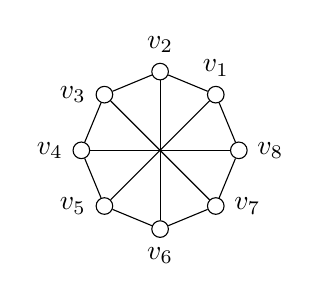
\begin{tikzpicture}
            \vertex (v1) at (45:1) [label=above:$v_1$]{};
            \vertex (v2) at (90:1) [label=above:$v_2$]{};
            \vertex (v3) at (135:1) [label=left:$v_3$]{};
            \vertex (v4) at (180:1) [label=left:$v_4$]{};
            \vertex (v5) at (225:1) [label=left:$v_5$]{};
            \vertex (v6) at (270:1) [label=below:$v_6$]{};
            \vertex (v7) at (315:1) [label=right:$v_7$]{};
            \vertex (v8) at (360:1) [label=right:$v_8$]{};
            
            \path 
            (v1) edge (v2)
            (v2) edge (v3)
            (v3) edge (v4)
            (v4) edge (v5)
            (v5) edge (v6)
            (v6) edge (v7)
            (v7) edge (v8)
            (v8) edge (v1)
            (v2) edge (v6)
            (v3) edge (v7)
            (v4) edge (v8)
            (v5) edge (v1)
            ;
        \end{tikzpicture}
        \end{center}
    \end{homeworkProblem}

    \begin{homeworkProblem}
        Let $G$ be a connected graph. For any two vertices $u$, $v$ let $d(u, v)$ be the distance from $u$ to $v$. Recall that the distance from $u$ to $v$ is the length of the shortest path from $u$ to $v$. 
        
        Prove the following triangle inequality. For all vertices $x$, $y$ and $z$ of the graph we have $d(x, z) \leq d(x, y) + d(y, z)$.

        \textbf{Solution:}
        Let's show this using a direct proof:

        If you simply connect the paths from $x$ to $y$ to the path connecting $y$ to $z$ you will
        have a valid path of length $d(x,y) + d(y,z)$. 

        However $d(x,y)+d(y,z)$ might not be the  \textit{shortest} path from $x \to z$, it could have a lot of cycles and detours and since by definition $d(x,z)$  will be a shorter or equidistant path from $x$ to $z$, this path will be shorter or equal than $d(x,y)+d(y,z)$ above and thus
        the triangle inequality will be satisfied.

        $\therefore d(x, z) \leq d(x, y) + d(y, z) \qed$ 

    \end{homeworkProblem}


    
    
    
    \end{document}